\documentclass{physlab}

\begin{document}
\begin{titlepage}
\center % Center everything on the page
 
%----------------------------------------------------------------------------------------
%	HEADING SECTIONS
%----------------------------------------------------------------------------------------

\textsc{\LARGE Московский\\[-0.2cm]Физико-Технический Институт\\[0.1cm]\large (государственный университет)}\\[1.5cm] % Name of your university/college
\textsc{\Large Кафедра общей физики}\\[0.1cm] % Major heading such as course name
\textsc{\large Лабораторная работа № 5.1}\\[0.5cm] % Minor heading such as course title

%----------------------------------------------------------------------------------------
%	TITLE SECTION
%----------------------------------------------------------------------------------------

\HRule
\\
{\huge \bfseries Измерение коэффициента ослабления \\[-3mm]
потока $\gamma$-лучей в веществе \\[3mm]
и определение их энергии}
\\[0.3cm] % Title of your document
\HRule
\\[1.5cm]


 
%----------------------------------------------------------------------------------------
%	AUTHOR SECTION
%----------------------------------------------------------------------------------------

\begin{minipage}[t]{0.48\textwidth}
	\begin{flushleft} \large
		\textsf{Студент}
		
		Ришат \textsc{Исхаков} \\[-0.15cm]
		512 группа

	\end{flushleft}
\end{minipage}
\hfill
\begin{minipage}[t]{0.48\textwidth}
	\begin{flushright} \large
		\textsf{Преподаватель}		
		
		Лев Владиславович \\[-0.15cm]
		\textsc{Инжечик} 

	\end{flushright}
\end{minipage}

\begin{bottompar}
	\begin{center}
		
\includegraphics[width = 80 mm]{logo.jpg}
	\end{center}
	\today

\end{bottompar}
\vfill % Fill the rest of the page with whitespace

\end{titlepage}

\paragraph{Цель работы:} С помощью сцинцтиляционного счётчика измеряются линейные коэффициенты ослабления потока $\gamma$-лучей  в свинце, железе и алюминии; по их величине определяется энергия $\gamma$-квантов.

\section{Теория}
Гамма-лучи возникают при переходе возбуждённых ядер в более низкое энергетическое состояние. Энергия $\gamma$-квантов обычно порядка ~$10\div1000$ кэВ. Заряд и масса $\gamma$-кванта равны нулю. Проходя через вещество, пучок $\gamma$-квантов ослабляется по закону:
\begin{equation}
    I = I_0e^{-\mu l}
\label{eq:coef}
\end{equation} 
	или
\begin{equation}
    I=I_0e^{-\mu' m_1},
\end{equation}
где $I, I_0$ - интенсивности прошедшего и падающего излучений, $l$~---~длина пути, пройденного  пучком $\gamma$-лучей, $m_1$~---~масса пройденного вещества на единицу площади, $\mu$ и $\mu'$~---~константы, зависящие от среды ($[\mu] = \text{см}^{-1}$, $[\mu'] = \text{см}^{2}/\text{г}$). $\mu'$, в отличие от $\mu$, не зависит от плотности среды. Ослабление потока $\gamma$-лучей в веществе связано с тремя эффектами: фотоэлектрическим поглощением, комптоновским рассеянием и генерацией электрон-позитронных пар.

\textbf{Фотоэлектричекое поглощение}

	При столкновении $\gamma$-квантов с электронами внутренних атомных оболочек может происходить поглощение квантов. Свободные (наружные) электроны не могут поглощать кванты.Вероятность $dP_\text{ф}$ фотоэлектрического поглощения $\gamma$-квантов: 
\[ dP_\text{ф}=\sigma_\text{ф} n_1 dl, \]
	где $dl$~---~длина пути, $n_1$~---~плотность внутренних  электронов, $\sigma_\text{ф}$~---~поперечное сечение фотоэлектрического поглощения.
\[ \mu_\text{ф}=\sigma_\text{ф}n_1, \]	
	$\mu_\text{ф}$~---~коэффициент поглощения для фотоэффекта $\mu$ из уравнения \eqref{eq:coef}.
	
	Фотоэффект является доминирующим механизмом поглощения $\gamma$-квантов при не очень высоких энергиях. Его вероятность зависит от энергии лучей и заряда  ядер.
\begin{figure}[H]
\centering
    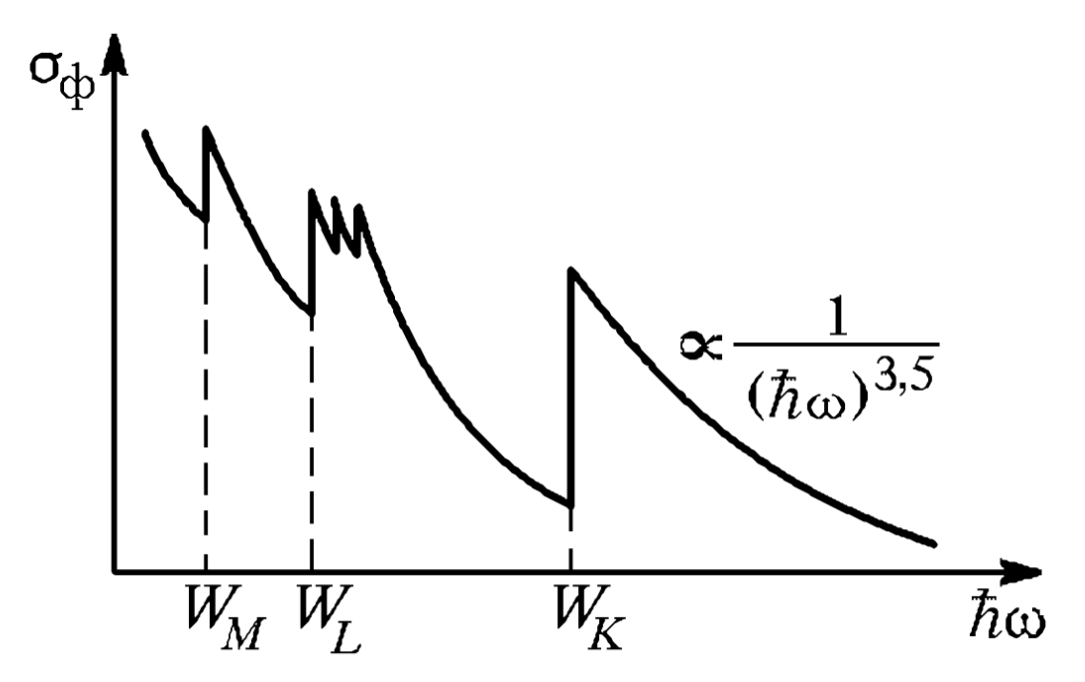
\includegraphics[width=0.45\linewidth]{01}
\caption{Зависимость сечения фотоэффекта от энергии $\gamma$-квантов.}
\end{figure}

\textbf{Комптоновское рассеяние}

Комптоновское рассеяние~---~упругое столкновение $\gamma$-кванта с электроном. Оно может происходить на свободных/слабосвязанных электронах. Эффект Комптона становится существенным, когда энергия квантов становится много больше энергии связи электронов в атоме. В этом случае сечение комптон-эффекта:
\begin{equation}
    \sigma_K=\pi r^2 \dfrac{mc^2}{\hbar \omega}\left(ln\frac{2\hbar\omega}{mc^2}+\frac{1}{2}\right),
\end{equation}
где $r\simeq 2.8 \cdot 10^{-13}$ см~---~классический радиус электрона, $m$~---~его масса.
	
Эффект комптона приводит не к поглощению, а к рассеянию $\gamma$-квантов и уменьшению их энергии.

\textbf{Образование пар}

При энергиях $\gamma$-лучей больше 1.02 МэВ становится возможным поглощение лучей, связанное с образованием электрон-позитронных пар. Оно возникает в электрическом поле ядер. Вероятность этого процесса приблизительно пропорциональна $Z^2$.
	   
\textbf{Полный коэффициент ослабления потока $\gamma$-лучей}
	 
Полный коэффициент ослабления потока лучей равен сумме коэффициентов для трёх рассмотренных процессов. 
	
\begin{figure}
\centering
    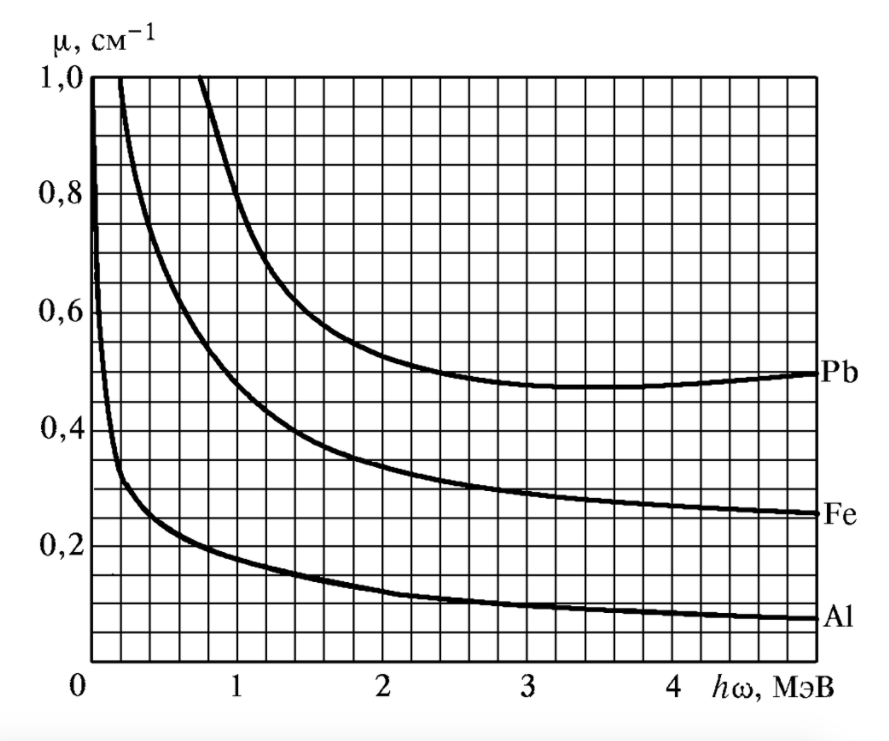
\includegraphics[width=0.5\linewidth]{02}
\caption{Полные коэффициенты ослабления потока $\gamma$-лучей в алюминии, железе и свинце.}
\end{figure}
	
 	Полный коэффициент ослабления:
 	
 	\begin{equation}
 	\mu=\frac{1}{l}ln\frac{N_0}{N}
 	\end{equation}
	
	В работе определяются толщина образца $l$, число падающих частиц $N_0$ и число прошедших частиц $N$.
	
\section{Экспериментальная установка}
	
\begin{figure} [h!]
	\centering
    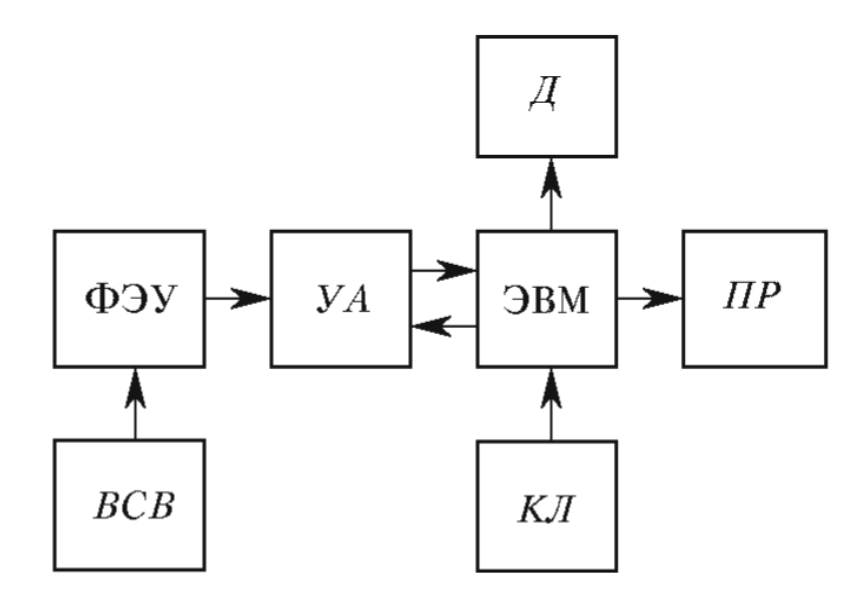
\includegraphics[width=0.8\linewidth]{03}
	\caption{Блок-схема установки, используемой для измерения коэффициентов ослабления потока $\gamma$-лучей; Pb~---~свинцовый контейнер с коллиматорным каналом; П~---~набор поглотителей, ПП~---~пересчётный прибор; С~---~сцинтиллятор (кристалл $NaI(Tl)$); ВВ~---~высоковольтный выпрямитель, Ф~---~формирователь-выпрямитель; И~---~источник $\gamma$-лучей}
\end{figure}

\begin{figure} [h!]
	\centering
	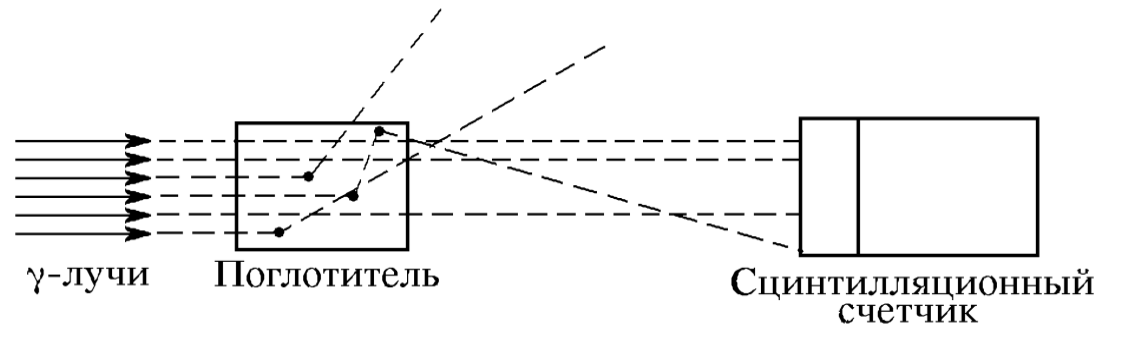
\includegraphics[width=0.9\linewidth]{04}
	\caption{Схема рассеяния $\gamma$-квантов в поглотителе}
\end{figure}
			
	

\section{Ход работы}
	
\begin{enumerate}
	\item Исследовали поглощение $\gamma$-лучей в свинце, железе и алюминии. Для этого измерили число частиц, попадающих в счётчик за фиксированное время  при различной толщине образцов (точность измерения $0.3\%$):  
		
	\begin{table}[H]
	\centering
		\caption{Результаты измерений для свинца:}
		\begin{tabular}{|c||c|c|c|c|c|}
			\hline
			$l$, мм & 4 & 8 & 12 & 16 & 20 \\ \hline
			$N$, шт. & 136746 & 102354 & 105008 & 104325 & 97589  \\ \hline
			$t_\Sigma$, с & 30 & 40 & 70 & 120 & 190 \\ \hline
		\end{tabular}
	\end{table}
		
	\begin{table}[H]
	\centering
		\caption{Результаты измерений для железа:}
		\begin{tabular}{|c||c|c|c|c|c|}
			\hline
			$l$, мм & 9 & 18 & 27 & 36 & 45 \\ \hline
			$N$, шт. & 136393 & 100156 & 112720 & 103385 & 98267 \\ \hline
			$t_\Sigma$, с & 30 & 40 & 80 & 130 & 220 \\ \hline
		\end{tabular}
	\end{table}
		
	\begin{table}[H]
    \centering
	   \caption{Результаты измерений для алюминия:}
	   \begin{tabular}{|c||c|c|c|c|c|}
			\hline
			$l$, мм & 20 & 40 & 60 & 80 & 100 \\ \hline
			$N$, шт. & 105329 & 102030 & 110819 & 100716 & 105235 \\ \hline
			$t_\Sigma$, с & 20 & 30 & 50 & 70 & 110 \\ \hline
		\end{tabular}
	\end{table}
		
	Абсолютная погрешность измерения толщины образца $\varepsilon_l=1$ мм.
    \item Измерили число частиц, попадающих в счётчик за фиксированное время в отсутствие поглотителя: \underline{$N_0=166505$} частиц \underline{за 20 секунд} (точность измерения 0,3\%). Чтобы учесть фон, обусловленный шумом ФЭУ и посторонними частицами, измерили количество частиц, попадающих на счётчик за фиксированное время при закрытии коллиматора свицовой заглушкой: \underline{$N_\text{фон.}=9986$} частиц \underline{за 400 секунд} (точность измерения $0.3\%$).
		Фон вычитается из всех результатов измерений.

\end{enumerate}
	
\section{Обработка данных}
\begin{enumerate}
	\item Построили графики зависимости $ln(N-N_\text{фон.}) = f(l)$ для всех исследуемых веществ:
	\begin{figure}[H]
		\begin{minipage}[h]{0.49\textwidth}
			\centering
			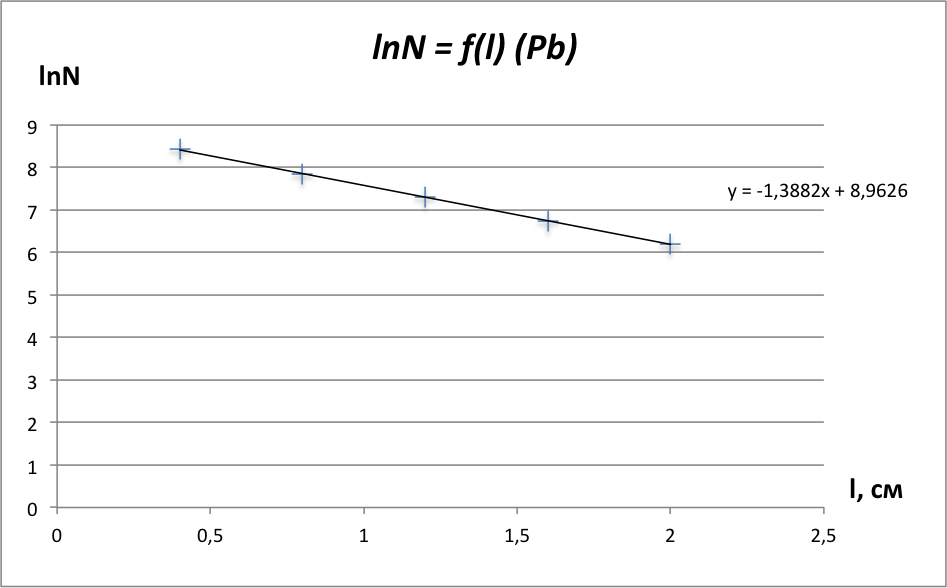
\includegraphics[width=1\linewidth]{05}
			\caption{График зависимости логарифма числа прошедших частиц от толщины образца для свинца}
		\end{minipage}
	\hfill
		\begin{minipage}[h]{0.49\textwidth}
			\centering
			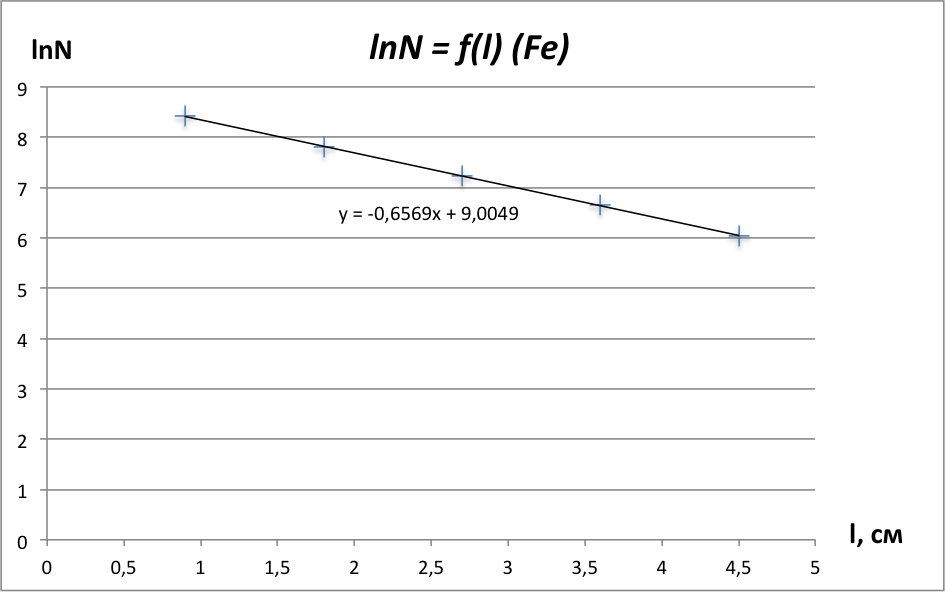
\includegraphics[width=1\textwidth]{06}
			\caption{График зависимости логарифма числа прошедших частиц от толщины образца для железа}
		\end{minipage}
	\end{figure}

	\begin{figure}[H]
		\centering
		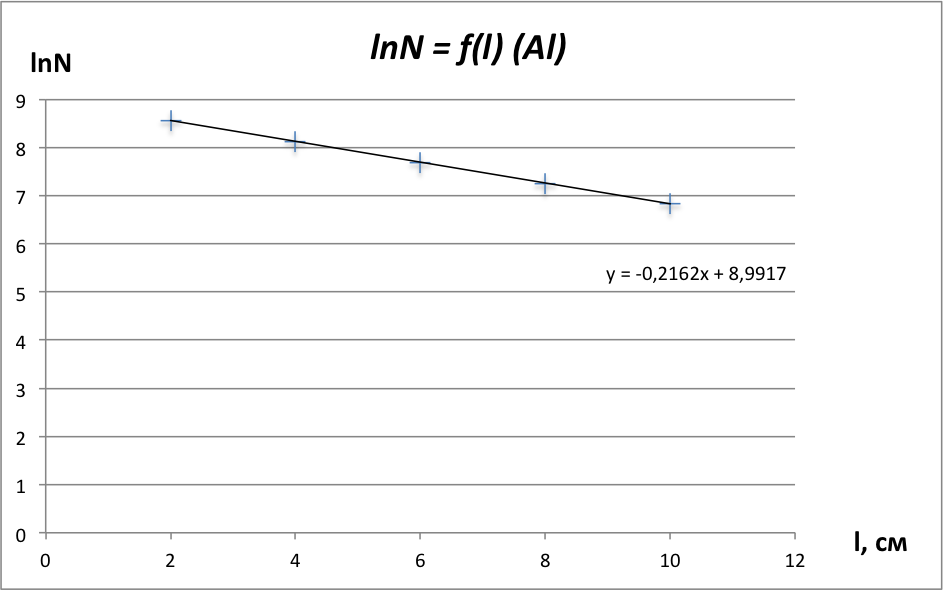
\includegraphics[width=0.6\linewidth]{07}
		\caption{График зависимости логарифма числа прошедших частиц от толщины образца для алюминия}
	\end{figure}
		
	\item С помощью графиков определили линейные коэффициенты ослабления для всех трёх веществ:
	\[ \mu_{Pb}\approx1,388 ~\text{см}^{-1} \]
	\[ \mu_{Fe}\approx0,657 ~\text{см}^{-1} \]
	\[ \mu_{Al}\approx0,216 ~\text{см}^{-1} \]
	
	\item По линейным коэффициентам ослабления нашли коэффициенты $\mu'$ по формулам (1) и (2):
	 
    \begin{equation}
	\text{Из (1) и (2)} \Rightarrow \mu l = \mu' m_1
	\end{equation}
	
	Отсюда:
    \[ \mu'_{Pb} \approx 0,122 ~\frac{\text{см}^2}{\text{г}} \]
	\[ \mu'_{Fe} \approx 0,084 ~\frac{\text{см}^2}{\text{г}} \]
	\[ \mu'_{Al} \approx 0,079 ~\frac{\text{см}^2}{\text{г}} \]
	
	\item Используя найденные коэффициенты ослабления и табличные данные, определили среднюю энергию $\gamma$-лучей, испускаемых источником:
	\[ E_{\gamma} \sim 0,5\div0,6 ~\text{МэВ} \]
		
	\item Рассчитали погрешности измерений:
    \begin{enumerate}
    %   \item Погрешность измерения толщины образцов:
    %	\[ l=1\text{мм} \]
        \item Погрешность построенных графиков, рассчитанная методом наименьших квадратов $(y=ax+b$):
        \[ \frac{da_1}{a_1} \approx 0,005 = 0,5\ \]
        \[ \frac{da_2}{a_2} \approx 0,004 = 0,4\ \]
        \[ \frac{da_3}{a_3} \approx 0,003 = 0,3\ \]
        
        \item С учётом погрешностей:
        \[ \mu_{Pb} = 1,388 \pm 0,007 ~\text{см}^{-1} \]
        \[ \mu_{Fe} = 0,657 \pm 0,003 ~\text{см}^{-1} \]
        \[ \mu_{Al} = 0,216 \pm 0,001 ~\text{см}^{-1} \]
	\end{enumerate}
		
\end{enumerate}
		
\section{Вывод} Исследовали поглощение $\gamma$-лучей в свинце, алюминии и железе. Получили линейные зависимости логарифма прошедших частиц от толщины образцов и по ним определили линейные коэффициенты ослабления $\mu$ и $\mu'$, а также среднюю энергию $\gamma$-лучей, испускаемых источником.  Полученное значение составило $E_{\gamma} \sim 0,5\div0,6 ~\text{МэВ}$. Погрешности измерений не превысили 1\%.

\end{document}